% 2013 年北京卷理科第 14 题：棱长为 2 的正方体 ABCD-A1B1C1D1。
% 来源 PDF：普通高考/2013/2013北京理.pdf，第 1 页（印面 787）中栏。
% E 为 BC 的中点，P 在线段 D1E 上。
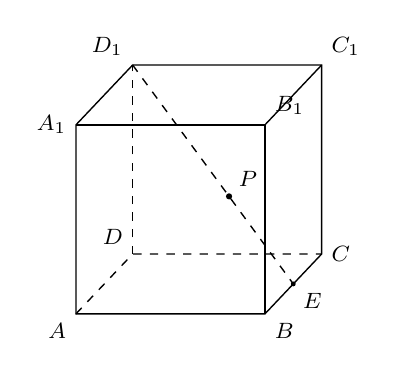
\begin{tikzpicture}[font=\footnotesize, line width=0.5pt, scale=0.8]
  % 前面 ABB1A1
  \coordinate (A) at (0,0);
  \coordinate (B) at (3,0);
  \coordinate (A1) at (0,3);
  \coordinate (B1) at (3,3);
  % 后面 DCC1D1（斜二测方向）
  \coordinate (D) at (0.9,0.95);
  \coordinate (C) at (3.9,0.95);
  \coordinate (C1) at (3.9,3.95);
  \coordinate (D1) at (0.9,3.95);
  % E 为 BC 中点
  \coordinate (E) at (3.45,0.475);
  % P 在线段 D1E 上
  \coordinate (P) at (2.43,1.865);
  % 可见棱
  \draw (A) -- (B) -- (C) -- (C1) -- (D1) -- (A1) -- cycle;
  \draw (A1) -- (B1) -- (B);
  \draw (B1) -- (C1);
  \draw (C) -- (C1);
  % 被遮挡的棱
  \draw[dashed] (A) -- (D) -- (C);
  \draw[dashed] (D) -- (D1);
  % 线段 D1E 与点 P
  \draw[dashed] (D1) -- (E);
  \fill (P) circle (1.4pt);
  \fill (E) circle (1.1pt);
  % 标签
  \node[below left] at (A) {$A$};
  \node[below right] at (B) {$B$};
  \node[right] at (C) {$C$};
  \node[above left] at (D) {$D$};
  \node[left] at (A1) {$A_1$};
  \node[above right] at (B1) {$B_1$};
  \node[above right] at (C1) {$C_1$};
  \node[above left] at (D1) {$D_1$};
  \node[below right] at (E) {$E$};
  \node[above right] at (P) {$P$};
\end{tikzpicture}
